\title{Documentation - Lagrangian part of the TMP-Code}
\author{Lukas Muessle}
\date{\today}
\documentclass[12pt]{article}

\usepackage{palatino} 	% use palatino as font
\usepackage{lipsum} 	% get some blindtext
\usepackage{placeins} 	% force floats into section
\usepackage{makecell}	% to center the tables
\usepackage[margin=2.5cm]{geometry}	% width of the text
\usepackage{seqsplit}	% split long words with \seqsplit{}
\usepackage{color}		% for \textcolor usage\
\usepackage{amsmath,amsfonts,amssymb,amscd,amsthm,xspace}
\usepackage{graphicx}

\begin{document}
\maketitle

%###################################################################
% Overview
%###################################################################
\section{Overview}
In this document you will find all information needed to use the Lagrangian part of the DNS-Code of the Turbulent Mixing Group(TMP) of the Max-Planck-Institute for Meteorology. The document is organized as follows, Section~\ref{sec:options} uses the initialization file "dns.ini" to explain the different option to run the Lagrangian part. Section~\ref{sec:interpolation} explains the interpolation method. Section~\ref{sec:statistics} presents the statistic tools. Section~\ref{sec:visualization} represents procedures for the visualization and Section~\ref{sec:tools} presents some useful shell tools.\newline
\textbf{Current status:} in progress \newline
\textbf{Last change:} March 2015
\newpage
%###################################################################
% Tables with options for dns.ini
%###################################################################
\section{Options for dns.ini}
\label{sec:options}
\subsection{Primary}
In the "[Main]" section of the file "dns.ini" the Lagrangian model can be activated using the flag "yes"' for the "CalculateParticle" option, the default value reads "no". Furthermore, the calculation method has to be set as shown in Table~\ref{tab:main}. 
\begin{table}
    \makebox[\textwidth][c]{\begin{tabular}{|l|l|l|}
    \hline
    \textbf{In [Main]}          & \textbf{Meaning }                          & \textbf{Option for value}    \\ \hline
    CalculateParticle & Switch on Lagrange part           & 'yes' or 'no'       \\ \hline
    Lagrange          & What kind of Lagrange calculation & see following Table~\ref{tab:type} \\ \hline
    \end{tabular}}
    \caption{Options which can be set in [Main] of "dns.ini".}
    \label{tab:main}
\end{table}
%\FloatBarrier
\subsection{Options for Lagrange initialize}
The different calculation methods for the Lagrangian model are listed in Table~\ref{tab:calc_methods}. Each setting defines the values for certain setup variables presented in Table~\ref{tab:setup_particles}. The according setups of this variables can be found in \seqsplit{"/lagrange/lagrange\_type\_initialize.f90"}. The first two types are self-explaining. The third option "SimpleSettling" subtracts a constant value of the vertical particle velocity in \seqsplit{"/lagrange/rhs\_particle\_global.f90"} with the flag \seqsplit{"LAG\_TYPE\_SIMPLE\_SETT"}. The following "BilinearCloud" options describe the liquid calculation for the Lagrangian model. The calculation are split over "/lagrange/rhs\_particle\_global.f90" and the according interpolation functions like \seqsplit{"/lagrange/rhs\_particle\_global\_interpolation.f90"}, \seqsplit{"/lagrange/rhs\_particle\_global\_interpolation\_halo\_1.f90"} and so on. We recommend using BilinearCloudThree for general liquid calculations as this option is the most accurate and fastest one. BilinearCloudFour uses the same method as BilinearCloudThree but with an additional scalar, which we use as a dummy to store the residence time information. To add a new calculation mode we can use the "search" alias introduced in Chapter~\ref{sec:tools}. For example, we can search for \seqsplit{"LAG\_TYPE\_BIL\_CLOUD\_4"} to see where we need to add new IF clause when implementing a new calculation method. More information according the residence times can be found in Chapter~\ref{sec:general_main}. \newline
\begin{table}
\label{tab:type}
    \makebox[\textwidth][c]{\begin{tabular}{|l|l|}
    \hline
    \textbf{Lagrange type}      & \textbf{Meaning}                                    \\ \hline
    None               & Lagrange module is switched off            \\ \hline
    Tracer             & Only tracers following the flow            \\ \hline
    SimpleSettling     & Simple settling                            \\ \hline
    BilinearCloud      & Simple combination of terms                          \\ \hline
    BilinearCloudTwo   & Second version of combination of terms                         \\ \hline
    BilinearCloudThree & Optimized calculation                      \\ \hline
    BilinearCloudFour  & Optimized calculation with residence times \\ \hline
    \end{tabular}}
    \caption{Options for the Lagrangian calculation method.}
    \label{tab:calc_methods}
\end{table}
The "Mixture" option needs to read "AirWaterBilinear" or "AirWaterBilinearStrat" to solve the liquid calculation in the Eulerian code. The calculation for "AirWaterBilinear" and "AirWaterBilinearStrat" can be found in \seqsplit{"/flow/flow\_buoyancy.f90"} and the setup in \seqsplit{"/thermodynamics/thermo\_initialize.f90"}. It is important to know that the third scalar of "AirWaterBilinearStrat" changes the index of scalars. This third scalar is used to create the stratification at the bottom of the domain. The buoyancy and liquid quantity is stored right after the general scalars. This leads to some IF statements at points inside the code where for example the liquid function is updated. To find these parts we can use the "search" alias introduced in Chapter~\ref{sec:tools} to search for \seqsplit{"MIXT\_TYPE\_BILAIRWATERSTRAT"}.
\begin{table}
    \makebox[\textwidth][c]{\begin{tabular}{|l|p{9cm}|p{4cm}|}
    \hline
    \textbf{Setup variable}           & \textbf{Meaning}                                                       & \textbf{Used for}                     \\ \hline
    inb\_particle\_evolution & Number of particle properties calculated time\_runge\_kutta.f90                 &  index particle array  \\ \hline
    inb\_particle\_aux       & Number of additional particle properties not looped in time\_runge\_kutta.f90   &  index particle array    \\ \hline
    inb\_particle\_txc       & Number of particle array for temporary calculation                              &  index particle array  \\ \hline
    inb\_lag\_aux\_field     & Number of Eulerian fields for Lagrangian (txc\_fields are used)                          & index Eulerian field array   \\ \hline
    inb\_particle            & Total number of particle properties (inb\_particle\_evolution + inb\_particle\_aux) &	 index particle array\\ \hline
    \end{tabular}}
    \caption{Setup variables for the particle properties. They are initialized in "modules/lagrange\_global.f90" and "modules/dns\_global.f90"}
    \label{tab:setup_particles}
\end{table}
%\FloatBarrier
\subsection{General options that need to be set}
\label{sec:general_main}
In this section we will describe the general setting that can be made for the Lagrangian scheme. All options are set in "[Lagrange]" and can be found in Table~\ref{tab:general}. The primary stats contain the total number of particles, the size of the particle array bumper and the initialization mode. The number of particles reads the total number of all simulated particles and the particle array bumper is used to safely communicate particles. \newline
The initialization mode features three options. The first option is to fill the whole domain randomly with particles, the second option is to fill a certain segment in y-direction. For both options we use the particle\_rnd\_mode=1, the Y\_Particle\_Pos and the Y\_Particle\_Width, which is the total width. As a third option, the particles can be distributed according to the first scalar(total water $q_t$) profile, where the value of the scalar profile is proportional to the particle density. For this option we use particle\_rnd\_mode=2 and a general limit of Jmax\_part and Jmin\_part so that particles are not initialized in the stretched regions.\newline
The amount of liquid that each particle features is determined in the function \seqsplit{"/tools/initialiaze/part/particle\_random\_position.f90"}. We use the function \seqsplit{"FIELD\_TO\_PARTICLE"} to interpolate the total water $q_t$ and the enthalpy $h$ scalars onto particle buffers and then calculate the liquid content according to the calculation in \seqsplit{"/flow/flow\_buoyancy.f90"} but only using the particle buffers with the interpolated scalar quantities instead of the actual scalars.\newline
We implemented a routine to plot trajectories. This routine saves the position data of some chosen particles for every iteration and outputs them together with the binary files. The current version of the trajectory routine \seqsplit{"/lagrange/dns\_write\_trajectories.f90"} reads a file, which contains the largest particles (see Chapter~\ref{sec:statistics}) and tracks these particular particles. To run the trajectories in the parallel mode there must be a minimum amount of particles, so that every processor features some particles. It is worth mentioning that the routine features the old version of the routine in the commented section at the end of the file. The old version of this routine would track every particle. \newline 
The dispersion option is an additional tool, which is not yet fully developed. It can be found in \seqsplit{"/tools/statistics/lagrange\_dispersion/"}. It is used to calculate the dispersion of particle pairs in time. \newline
The most important statistic tool is the particle PDF calculations. By default we set up an area over the whole horizontal domain and a span in the vertical direction using \seqsplit{"Y\_particle\_PDF\_pos"} and \seqsplit{"Y\_particle\_PDF\_width"}. The horizontal domain can be constrained with \seqsplit{"X\_particle\_PDF\_pos"}, \seqsplit{"Z\_particle\_PDF\_pos"}, \seqsplit{"X\_particle\_PDF\_width"} and \seqsplit{"Z\_particle\_PDF\_width"}, if desired. Using \seqsplit{"Particle\_PDF\_Max"} we can choose the maximum size of the bins according to the liquid field. The size of each bin is set by \seqsplit{"Particle\_PDF\_Interval"}. \newline
As already mentioned above, we created a tool, which measures the residence time using BilinearCloudFour. This tool uses an additional part of the l\_q and l\_hq array. This workaround is used to make sure the residence time for each particle are properly communicated. We use the last part of the l\_q array to safe the residence time for particles in the range of 2 $\times$ lambda at the cloud top and the l\_hq for half of the cloud domain. We use the variable l\_y\_lambda and l\_y\_base for this threshold, the setup of these variables can be found in \seqsplit{"/tools/dns/dns\_main.f90"}. Every time-step in \seqsplit{"/tools/dns/time\_integration.f90"} we calculate the residence times for every particle by adding up the time-steps, therefore we check the location inside the domain and calculate the different residence time for the 2 $\times$ lambda and half of the cloud domain. The residence time of a cloud droplet, which is beneath half of the cloud domain, will be set to zero. Therefore, we account for cloud droplets, which have a great chance to leave the cloud a the cloud base. If it is necessary to continue an old residence measurement it is important to flag \seqsplit{"ResidenceReset"} with "no", because the default value resets the residence times. Unfortunately the restart of the residence time measurements can only be done for the particles staying in the l\_y\_lambda region as the l\_hq array(buffer for half of the domain residence times) is not saved with the output routine. \newline
The Parameter option is implemented for future studies. Right now it is only used for the settling parameter. The "lagrange\_param is allocated in \seqsplit{"/modules/lagrange\_global.f90"}.
\begin{table}
    \makebox[\textwidth][c]{\begin{tabular}{|p{4cm}|p{6cm}|p{5cm}|}
    \hline
    \textbf{In [Lagrange]    }           & \textbf{Meaning }                                                 & \textbf{Option for value}                                               \\ \hline
    particle\_number                     & Amount of particles                                               & number                                                              \\ %\hline
     particle\_bumper                     & bumper for size of isize\_particle                                & number                                                             \\ %\hline
    particle\_rnd\_mode                  & Which mode of initialization                                      & 1 = random distribution in y-direciton, 2 = use scalar profile \\ \hline
        Y\_Particle\_Pos, Y\_Particle\_Width & Boundary values for particle\_rnd\_mode=1                                & in percentage                                                  \\ %\hline
        Jmax\_part, Jmin\_part               & Boundary values for particle\_rnd\_mode=2                                & in grid units                                                  \\ \hline
    CalculateTrajectories                & Should trajectories be calculated                                 & 'yes' or 'no'                                                  \\ %\hline
    Num\_trajectories                    & How many trajectories                                             & number                                                         \\ %\hline
    Num\_dispersion                      & number of pairs for the statistic tool of dispersion of particles & number                                                             \\ \hline
    CalculateParticlePDF                 & Should the particle PDF be calculated                             & 'yes' or 'no'                                                  \\ %\hline
    Y\_particle\_PDF\_pos                & Area for PDF (Y)                                                  & percentage                                                     \\ %\hline
    Y\_particle\_PDF\_width              & ~                                                                 & "                                                              \\ %\hline
    X\_particle\_PDF\_pos                & Area for PDF (X) - default off                                    & "                                                              \\ %\hline
    X\_particle\_PDF\_width              & ~                                                                 & "                                                              \\ %\hline
    Z\_particle\_PDF\_pos                & Area for PDF (Z) - default off                                    & "                                                              \\ %\hline
    Z\_particle\_PDF\_width              & ~                                                                 & "                                                              \\ %\hline
    Particle\_PDF\_Max                   & Maximum bin for liquid                                         & value                                                          \\ %\hline
    Particle\_PDF\_Interval              & Size of each bin                                               & value                                                          \\ \hline
    ResidenceReset                       & Reset residence timer                                             & 'yes' or 'no' - default 'yes'                                  \\ \hline
    Parameter                            & Parameters, for example settling                                  & amount of parameters                                           \\ \hline
    \end{tabular}} 
    \caption{General setup variables for the Lagrangian scheme}
    \label{tab:general}   
\end{table}
%\FloatBarrier
%###################################################################
% Interpolation
%###################################################################
\section{Interpolation algorithm}
\label{sec:interpolation}
To interpolate the data between the field and the Lagrangian scheme, we developed three main functions. The first takes care of the right hand side calculation for all given scalars. The second interpolates only one Eulerian scalar field to the particles inside the domain. The third routine does exactly the opposite, the particle information is extrapolated to the surrounding grid point. In the following section we will discuss the RHS algorithm, which can be found in \seqsplit{"/lagrange/rhs\_particle\_global\_interpolation.f90"}, \seqsplit{"/lagrange/rhs\_particle\_global\_interpolation\_halo\_1.f90"} and so on. The second and third routines can be found in \seqsplit{"/lagrange/field\_to\_particle.f90"} and \seqsplit{"/lagrange/particle\_to\_field.f90"}. These two routines will be explained in a second section after the right hand side. To get a brief overview of all functions we present a roadmap in Figure~\ref{fig:roadmap} at the end of the document. 
\subsection{RHS}
Before explaining the actual interpolation algorithm we will give an overview about the arrays you need hand over to the subroutines to use the RHS interpolation. \seqsplit{"/lagrange/rhs\_particle\_global\_interpolation.f90"} needs:
\begin{itemize}
	\item [\textbf{Input}]
	\item q [Eulerian fields] $\rightarrow$ information for interpolation
	\item l\_q [Particle property] $\rightarrow$ used to calculate local grid position
	\item y [Grid] $\rightarrow$ used to calculate local grid position
	\item wrk1d [1D-Buffer] $\rightarrow$ used for scaling (defined in rhs\_particle\_global.f90)
	\item txc [Eulerian buffer field] $\rightarrow$ dummy for liquid calculation
	\item grid\_start [Number] $\rightarrow$ start value in particle array for particles belonging to grid zone (defined in rhs\_particle\_global.f90)
	\item grid\_field\_counter [Number] $\rightarrow$ end value in particle array for in grid zone (defined in rhs\_particle\_global.f90)
	\item [\textbf{Output}]
	\item l\_hq [Particle tendencies] $\rightarrow$ here we update the particle tendencies
\end{itemize}
The subroutines for the halo zones take the "halo fields" instead of "q" and a different start and end position inside the particle array.\newline
The interpolation of the tendencies from the Eulerian scheme to the Lagrangian particle position is fulfilled with a trilinear interpolation which reads
\begin{equation}
\begin{split}
f_{\vec{X_i}}(\vec{v},\vec{q_j}) \approx f(\vec{p}_{111})(x_2-X)(y_2-Y)(z_2-Z)
+f(\vec{p}_{211})(X-x_1)(y_2-Y)(z_2-Z)\\
+f(\vec{p}_{121})(x_2-X)(Y-y_2)(z_2-Z)
+f(\vec{p}_{221})(X-x_1)(Y-y_1)(z_2-Z)\\
+f(\vec{p}_{112})(x_2-X)(y_2-Y)(Z-z_1)
+f(\vec{p}_{212})(X-x_1)(Y_2-y)(Z-z_1)\\
+f(\vec{p}_{122})(x_2-X)(Y-y_1)(Z-z_1)
+f(\vec{p}_{222})(X-x_1)(Y-y_1)(Z-z_1),
\end{split}
\label{eqn:interpolation}
\end{equation}
where $X$, $Y$ and $Z$ are the position of the particle, embedded by $x_{1}$, $x_{2}$, $y_{1}$, $y_{2}$, $z_{1}$ and $z_{2}$ the grid points and $\vec{p}_{abc}=(x_a, y_b, z_c)$ represents the quantity at the grid points. The interpolation is sketched in a two-dimensional setup in Figure~\ref{fig:interpolation_sketch}, where the black rectangles represent the Eulerian grid points and the blue point represents the Lagrangian particle.
\begin{figure}[htbp]
	\centering
		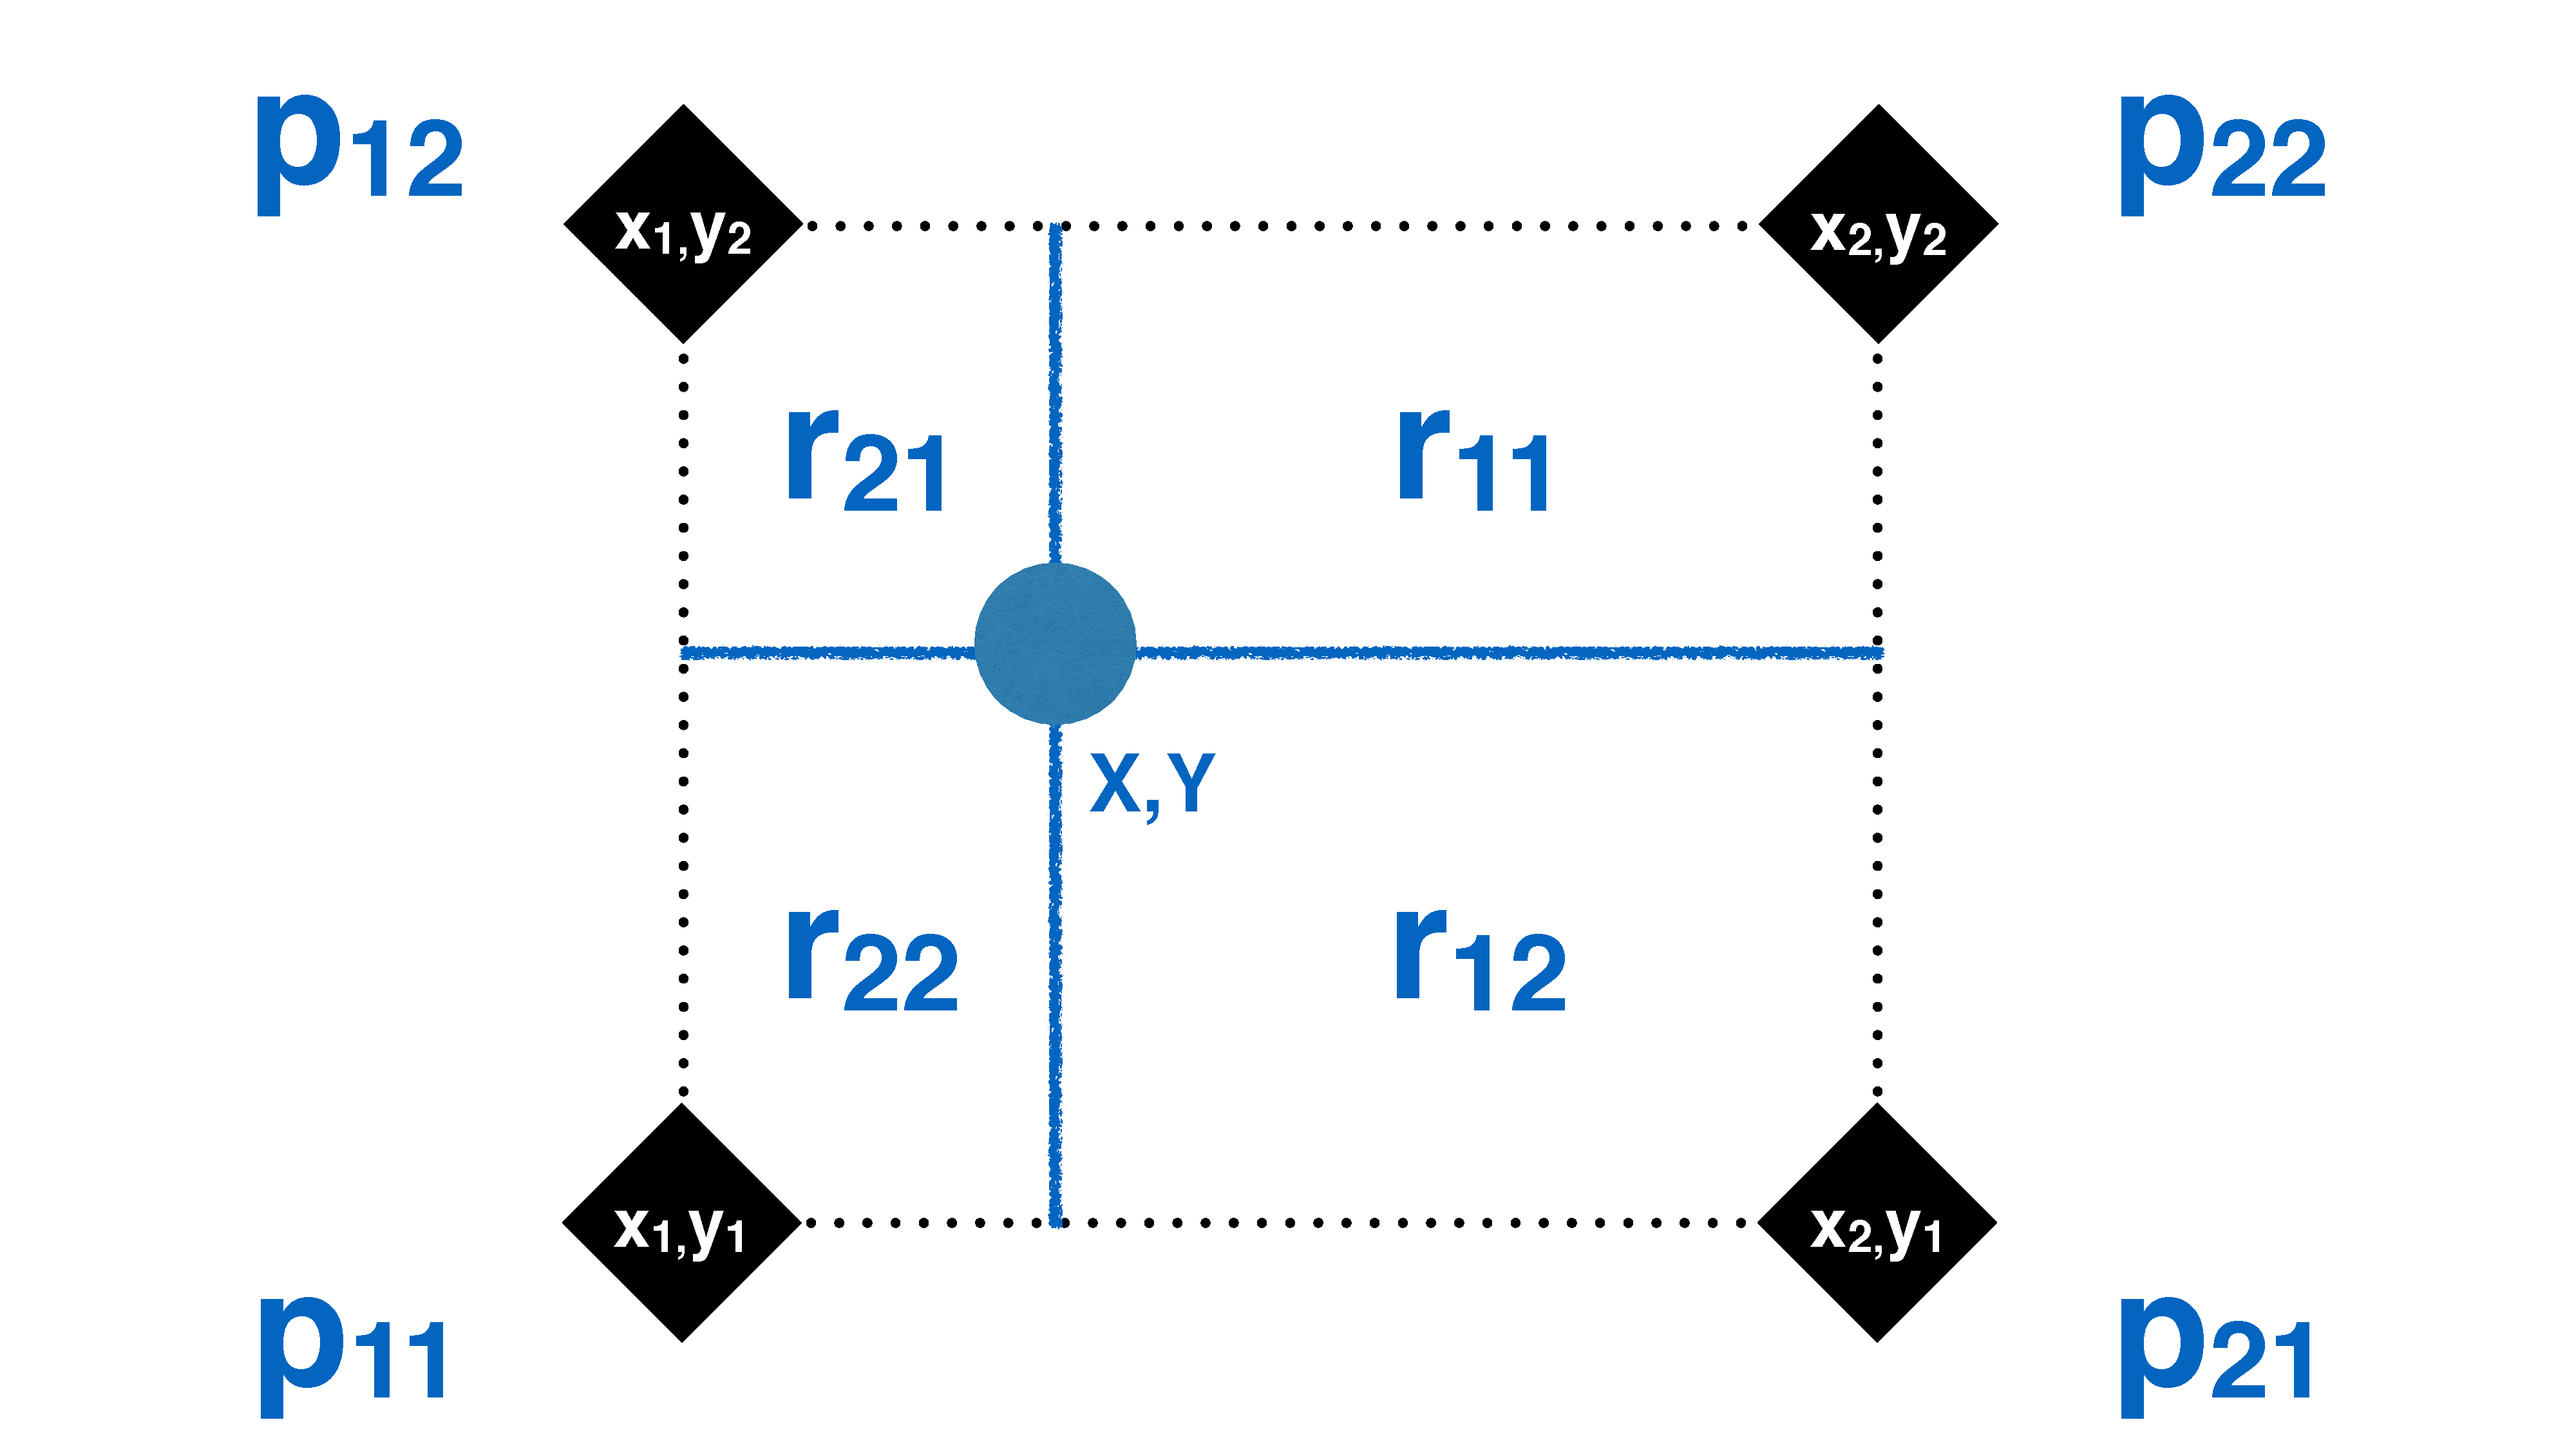
\includegraphics[width=0.8\textwidth,height=0.8\textheight,keepaspectratio]{figs/interpolation_sketch.pdf}
%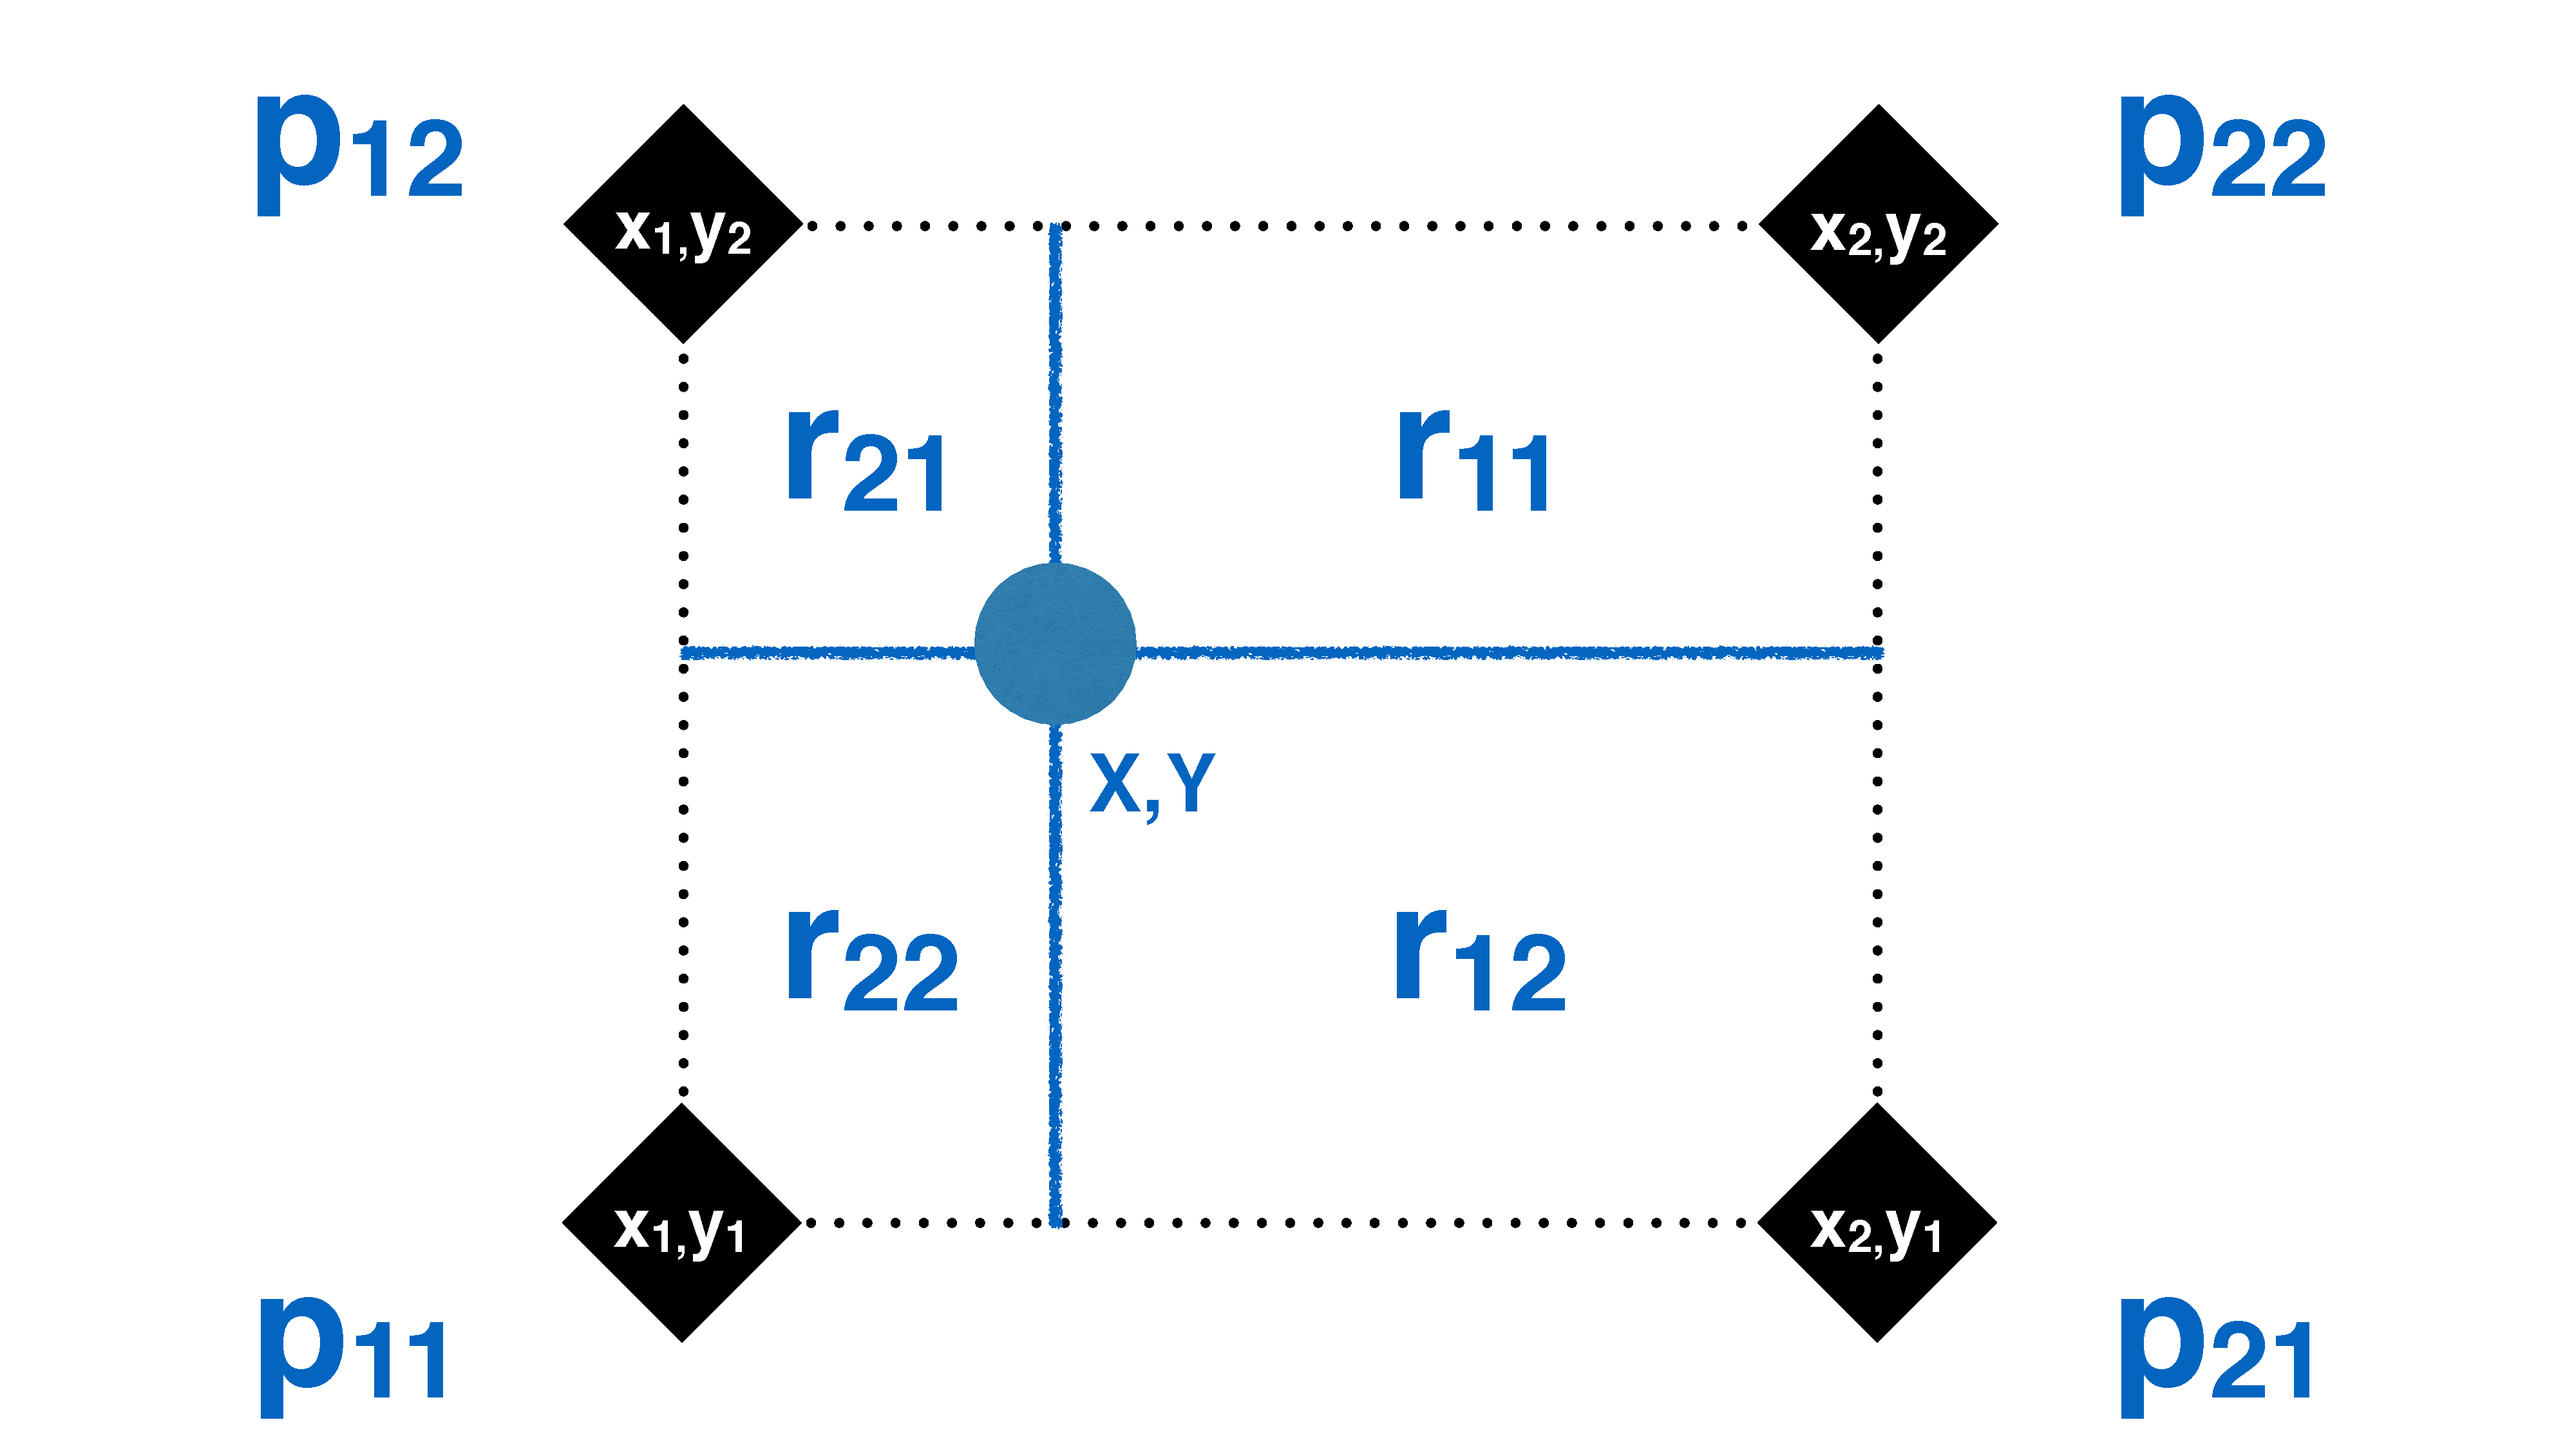
\includegraphics[width=\textwidth,height=\textheight]{figs/interpolation_sketch.pdf}
	\caption[Interpolation sketch]{This sketch clarifies the interpolation procedure. The black rectangles represent the Eulerian grid points, whereas the blue point, represents a Lagrangian parcel or particle. The tendencies of the quantities are interpolated for the position of the blue point inside the grid using the calculated rectangles $r_{ab}$.}
	\label{fig:interpolation_sketch}
\end{figure}
For simplicity, the sketch only represents a bilinear interpolation, whereas for a trilinear interpolation a third dimension would be present. The interpolated quantities $p_{ab}$ are weighted by the corresponding rectangles $r_{ab}$ on the opposite side of $p_{ab}$ and then summed up to be used as the interpolated quantity for the particles. \newline
However, the trilinear interpolation has its limit at transitions regions at the boundary of the cloud-top. Steep gradients lead to interpolation errors, so that expressions with expected steep gradients are calculated for each particle individually to minimize the interpolation error. 
\subsection{Field to particle and vice versa}
As mentioned above, we have a second tool to interpolate only a single scalar field to a particle quantity using \seqsplit{"/lagrange/field\_to\_particle.f90"}. This subroutine uses the subroutines for the development of the halo zones, the sorting algorithm and the right hand side interpolation for only one scalar. This subroutine needs:
\begin{itemize}
	\item [\textbf{Input}]
	\item scalar field [Eulerian field] $\rightarrow$ information for interpolation
	\item wrk1d [1D-Buffer] $\rightarrow$ used for scaling 
	\item wrk2d [2D-Buffer] $\rightarrow$ used for halo\_plane\_shifting
	\item wrk3d [3D-Buffer] $\rightarrow$ used for halo\_plane\_shifting
	\item x [Grid] $\rightarrow$ information for particle\_sort
	\item y [Grid] $\rightarrow$ used for scaling
	\item z [Grid] $\rightarrow$ information for particle\_sort
	\item l\_tags [Particle ID] $\rightarrow$ for particle\_sort
	\item l\_hq [Particle tendencies] $\rightarrow$ for particle\_sort
	\item l\_q [Particle properties] $\rightarrow$ to determine local grid position for interpolation and for particle\_sort
	\item [\textbf{Output}]
	\item particle\_property [Buffer] $\rightarrow$ here we store the interpolated values
\end{itemize}
For the particle\_property we mainly use l\_txc.\newline
The third subroutine extrapolates a particle quantity back to a field. The interpolation algorithm is customized in a way that the particle information is extrapolated to the eight surrounding grid points, using the trilinear interpolation explained above. The so constructed fields have the same structure as the scalar fields of the Eulerian scheme, so that all statistic tools of the Eulerian scheme can be used on those fields. The subroutine \seqsplit{"/lagrange/particle\_to\_field.f90"} is split into the actual interpolation using \seqsplit{"/lagrange/rhs\_particle\_to\_field.f90"} and the sending of the information using \seqsplit{"/lagrange/particle\_to\_field\_send\_recv\_east.f90"} and \seqsplit{"/lagrange/particle\_to\_field\_send\_recv\_north.f90"}. The general subroutine needs:
\begin{itemize}
	\item [\textbf{Input}]
	\item l\_q [Particle properties] $\rightarrow$ particle position for interpolation
	\item particle\_property [] $\rightarrow$ particular particle property we extrapolate to the field 
	\item x [Grid] $\rightarrow$ not yet used
	\item y [Grid] $\rightarrow$ used for scaling
	\item z [Grid] $\rightarrow$ not yet used
	\item wrk1d [1D-Buffer] $\rightarrow$ used for scaling
	\item wrk2d [3D-Buffer] $\rightarrow$ used for particle\_to\_field\_send\_recv
	\item wrk3d [3D-Buffer] $\rightarrow$ used for particle\_to\_field\_send\_recv
	\item [\textbf{Output}]
	\item field\_out [Eulerian field] $\rightarrow$ here we store the extrapolated field
	\end{itemize}
%\FloatBarrier
%###################################################################
% Statistics
%###################################################################
\section{Statistics}
\label{sec:statistics}
\subsection{Fields}
All statistic files are processed with the program "tkstat". We implemented two additional "avg" files, which contains the extrapolated field data from the liquid calculation with and without the diffusion term. The Lagrangian files have the index $x = n+l$, where n is the amount of produced avg-files of the eulerian scheme and l=1 is the liquid field with the diffusion term and l=2 the calculation without the diffusion term. \newline
Generally speaking, we have both liquid quantities on avg5s and avg6s, except when we use "AirWaterBilinearStrat". There we have 3 general scalars, which set the buoyancy and liquid field on avg4s and avg5s and the Lagrangian ones to avg6s and avg7s.
\subsection{Tools}
The folder \seqsplit{"/tools/statistics/"} contains some additional Lagrangian tools. Most of these tools are in a developing stage. We already mentioned \seqsplit{"lagrange\_dispersion"} and \seqsplit{"lagrange\_pdf"}. \newline
The tool \seqsplit{"lagrange\_trajec"} is used as a post processing tool to calculate the largest cloud droplets, the information are stored in a file called "largest\_particle". To find the position of these largest cloud droplets at the start of the simulation, we use \seqsplit{"lagrange\_pos\_trajec"}. The data is saved in a file called \seqsplit{"pos\_largest\_particle\_start"}, which is used by \seqsplit{"lagrange\_ini\_trajec"} to sort these largest particles to the beginning of the particle array as we want to start the simulation again with less particles to track the largest ones for every time-step. These three post processing tools are not fully developed and need to be treated with caution. We discovered that the exact reproduction of the largest trajectories is yet not possible due to some random calculations in the pressure solver in the parallel mode.
%###################################################################
% Visualization
%###################################################################
\section{Visualization}
\label{sec:visualization}
For the visualization we used the DNS tool "ensight" and the visualization programs Paraview and Avizo. We use the tool ensight to create files which can be used with Paraview and Avizo. Inside ensight we use the "particle\_to\_field" routine to create a general density field of particles and two fields according to the two liquid fields we calculated for the Lagrangian scheme. In the newer versions of the DNS code ensight might be referred as visuals. \newline
For Paraview we use the Format=1 and mainly a slide of the simulation cube. Additionally, we use Paraview to visualize the trajectory data. Therefore, we need to read the different trajectory data as "\textbf{VTK Particle Files"}. It is important that the option \textbf{"Has Scalar"} in the Paraview \textbf{Properties} window is unchecked. To track the particles inside Paraview we add the \textbf{Filter} "Temporal Particles To Pathlines" with Mask Points=1, this filter was working with Paraview version 4.3.1. In the Properties window of the path lines we can choose a solid color for the path lines to differentiate between different trajectories. To follow particular trajectories inside the domain it is helpful to go to \textbf{View} and check \textbf{Animation View}. In the Animation window we can first choose \textbf{Real Time} in the \textbf{Mode} section. The \textbf{Duration} on the right side of the \textbf{Animation View} determines the \textbf{Real Time}. Then we want to track a particular trajectory, therefore we need to have a single trajectory data loaded. We click on the actual data vector in the \textbf{Pipeline Browser} (its the actual name of the data we loaded), then we need to add a new \textbf{Camera} in the \textbf{Animation View} panel and we choose \textbf{Follow Data}. After we zoomed to our Data, we can now start the animation with the \textbf{Play} button. To create movies we used \textbf{Save Animation} and combined the .png pictures with a small program (Adapter for OS X) to a movie. To visualize groups or single particles we used the program called "extract\_trajec.py", which creates additional .vtk files. \newline
For Avizo we basically used a cube where the Subdomain=1,1024,740,840,1,1024 and the Format=2. The Avizo raw files need to be in the .nc format. To create the .nc file we use a small python program, which can be found in the documentation folder and is called "nc\_gen.py".
%###################################################################
% Tools
%###################################################################
\section{Useful tools}
\label{sec:tools}
\FloatBarrier
In this section, we present some useful tools to understand and work with the code. The following tools are aliases for the shell. 
\begin{itemize}
	\item search 'foobar' = \begin{verbatim}alias search 'grep -r --color --include="*.f90" \!^ .' \end{verbatim}
	\item h\_search 'foobar' = \begin{verbatim}alias h_search 'grep -r --color --include="*.h" \!^ .'	 \end{verbatim}
	\item txt\_search 'foobar' = \begin{verbatim}alias txt_search 'grep -r --color --include="*.txt" \!^ .' \end{verbatim}
\end{itemize}
The 'search' command digs recursivly through all *.f90 files, and the "h\_search" through all *.h and the "txt\_search" through all *.txt files.
%\FloatBarrier
%###################################################################
% Sketch
%###################################################################
%\section{Appendix}
%\label{sec:appendix}
\begin{figure}[htbp]
	\centering
			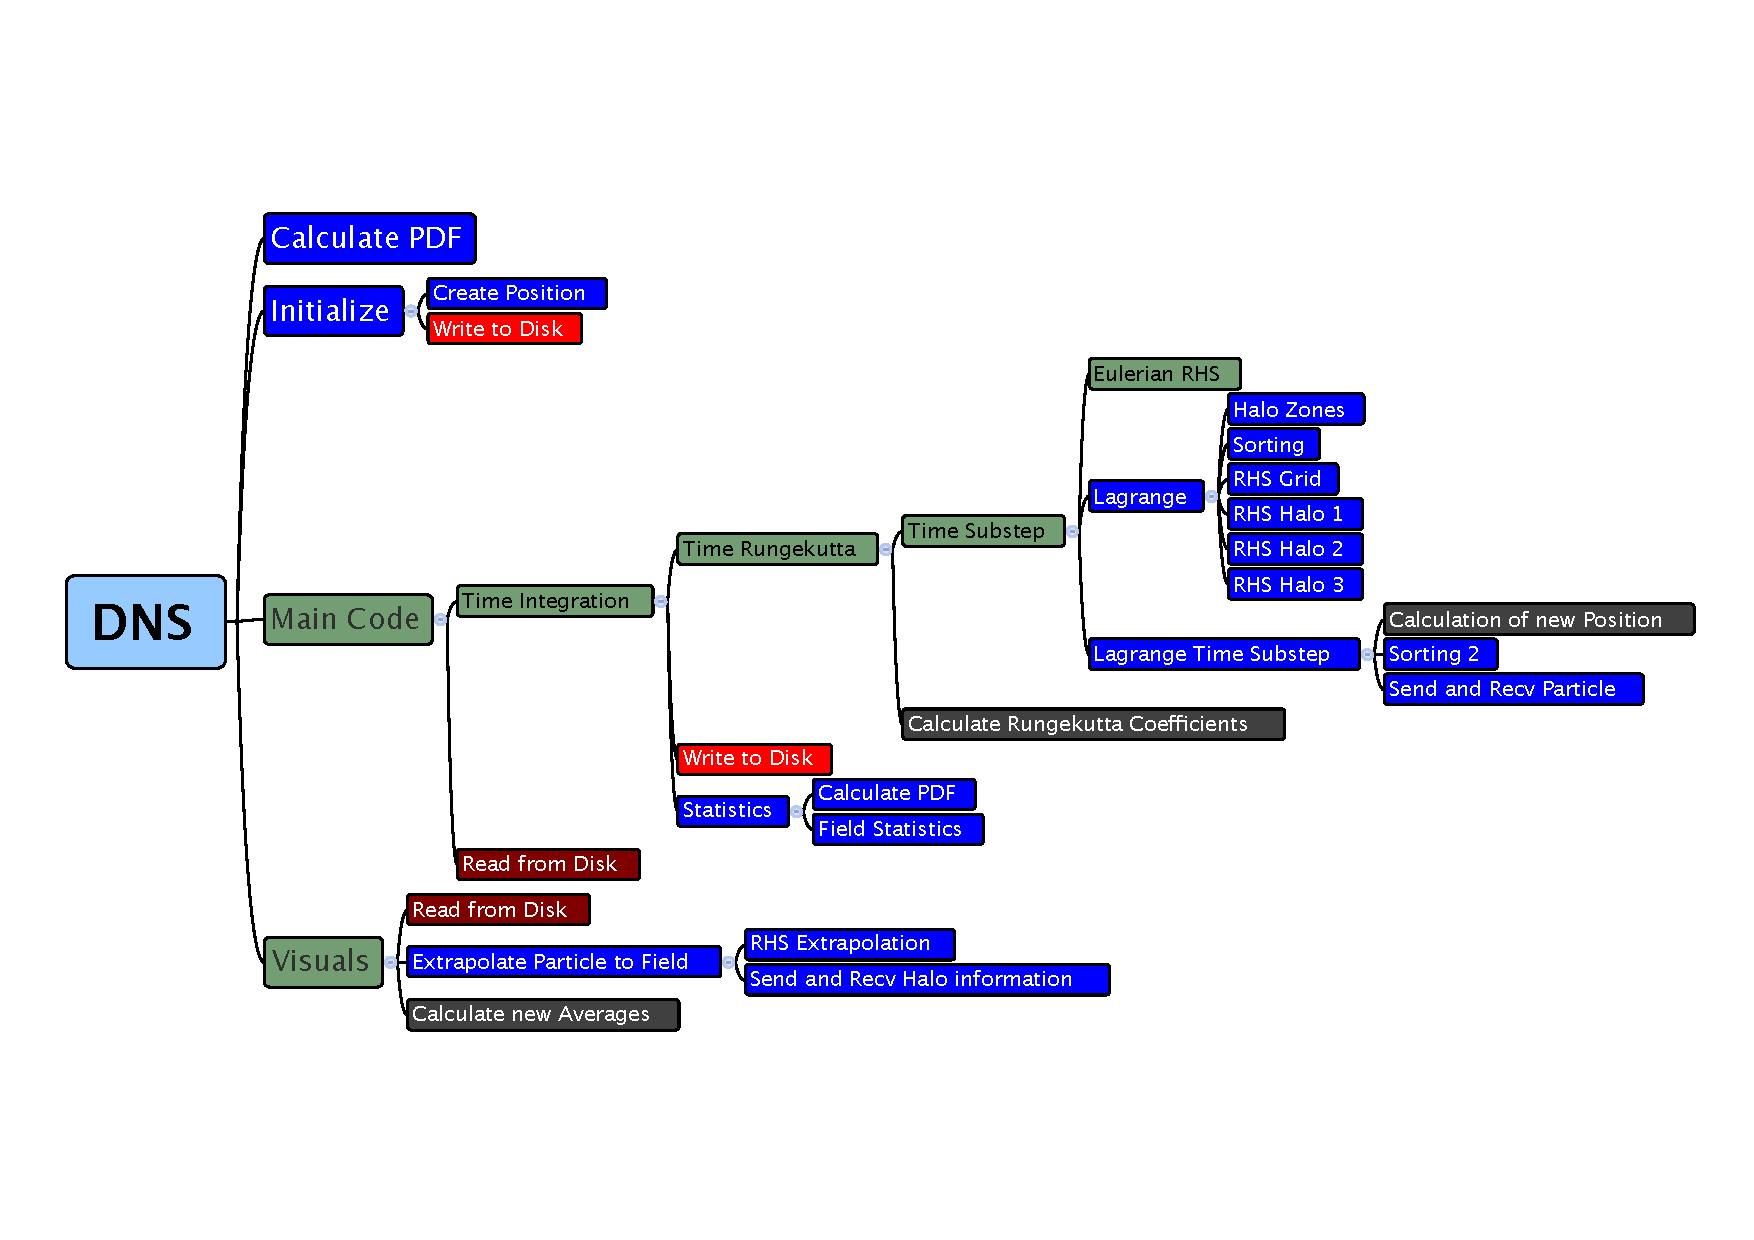
\includegraphics[width=\textheight,height=\textwidth, angle=90]{figs/latex_roadmap.pdf}
%        	\includegraphics[width=\textwidth,height=\textheight,keepaspectratio]{figs/roadmap_table.pdf}
	\caption[Implementation flow chart]{Simplified flow chart of functions used for the Lagrangian implementation. Green colors indicate Eulerian functions, blue represent the Lagrangian functions, red the Lagrangian I/O functions and the dark grey color indicates added calculation inside existing functions.}
	\label{fig:roadmap}
\end{figure}

%\FloatBarrier
\end{document}
